\documentclass[journal,12pt,onecolumn]{IEEEtran}
\usepackage{cite}
\usepackage{graphicx}
\usepackage{amsmath,amssymb,amsfonts,amsthm}
\usepackage{algorithmic}
\usepackage{graphicx}
\usepackage{textcomp}
\usepackage{xcolor}
\usepackage{txfonts}
\usepackage{listings}
\usepackage{enumitem}
\usepackage{mathtools}
\usepackage{gensymb}
\usepackage{comment}
\usepackage[breaklinks=true]{hyperref}
\usepackage{tkz-euclide} 
\usepackage{listings}
\usepackage{gvv}                                        
%\def\inputGnumericTable{}                                 
\usepackage[latin1]{inputenc} 
\usetikzlibrary{arrows.meta, positioning}
\usepackage{xparse}
\usepackage{color}                                            
\usepackage{array}                                            
\usepackage{longtable}                                       
\usepackage{calc}                                             
\usepackage{multirow}
\usepackage{multicol}
\usepackage{hhline}                                           
\usepackage{ifthen}                                           
\usepackage{lscape}
\usepackage{tabularx}
\usepackage{array}
\usepackage{float}
\newtheorem{theorem}{Theorem}[section]
\newtheorem{problem}{Problem}
\newtheorem{proposition}{Proposition}[section]
\newtheorem{lemma}{Lemma}[section]
\newtheorem{corollary}[theorem]{Corollary}
\newtheorem{example}{Example}[section]
\newtheorem{definition}[problem]{Definition}
\newcommand{\BEQA}{\begin{eqnarray}}
\newcommand{\EEQA}{\end{eqnarray}}
\usepackage{float}
%\newcommand{\define}{\stackrel{\triangle}{=}}
\theoremstyle{remark}
\usepackage{circuitikz}
\usepackage{tikz}

\title{IN  INSTRUMENTATION ENGINEERING}
\author{EE25BTECH11031- Sai Sreevallabh}

\author{Sai Sreevallabh - ee25btech11031}

\begin{document}

\maketitle
\section*{\textbf{Q.1-Q.20 Carry one mark each}} 

\begin{enumerate}
% Q1
\item If $v$ is a non-zero vector of dimension $3\times 1$, then the matrix
$A = vv^T$ has a rank = \rule{1.5cm}{0.4pt} \par \hfill\brak{\text{GATE IN 2017}}


% Q2
\item \figref{fig:placeholder_1} shows a shape ABC and its mirror image $A_1B_1C_1$ across the horizontal axis (X-axis). 
The coordinate transformation matrix that maps $ABC$ to $A_1B_1C_1$ is 
\begin{figure}[H]
    \centering
    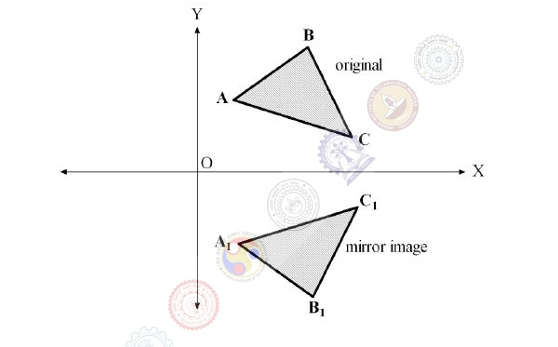
\includegraphics[width=0.5\columnwidth]{Figs/Q-2.png}
    \caption{Mirror Image across horizontal axis}
    \label{fig:placeholder_1}
\end{figure}
\par \hfill\brak{\text{GATE IN 2017}}
\begin{enumerate}
\begin{multicols}{2}
    \item $\myvec{0 & 1 \\ 1 & 0}$
    \item $\myvec{-1 & 0 \\ 1 & 0}$
    \item $\myvec{0 & 1 \\ -1 & 0}$
    \item $\myvec{0 & -1 \\ 1 & 0}$
\end{multicols}
\end{enumerate}

% Q3
\item Let $z=x+j y$ where $j = \sqrt{-1}$. Then $\cos z$ =\par \hfill\brak{\text{GATE IN 2017}}
\begin{enumerate}
\begin{multicols}{4}
    \item $\cos z$
    \item $\cos \bar{z}$
    \item $\sin z$
    \item $\sin \bar{z}$
\end{multicols}
\end{enumerate}

% Q4
\item The eigenvalues of the matrix 
$A = \myvec{1 & -1 & 5 \\ 0 & 5 & 6 \\ 0 & -6 & 5 }$
are  \par \hfill\brak{\text{GATE IN 2017}}
\begin{enumerate}
\begin{multicols}{4}
    \item $-1, 5, 6$
    \item $1, -5 \pm j6$
    \item $1, 5 \pm j6$
    \item $1, 5, 5$    
\end{multicols}
\end{enumerate}

% Q5
\item For a first order lowpass filter with unity d.c. gain and $-3\text{dB}$ corner frequency of $2000\pi$ rad/s, the transfer function $H\brak{j\omega}$ is \par \hfill\brak{\text{GATE IN 2017}}
\begin{enumerate}
\begin{multicols}{4}
    \item $\frac{1}{1 + j 1000 \omega}$
    \item $\frac{2000\pi}{2000\pi + j\omega}$
    \item $\frac{1}{1 + j\omega/(2000\pi)}$
    \item $\frac{1000}{1000 + j\omega}$
\end{multicols}
\end{enumerate}

% Q6
\item A series R-L-C circuit is excited with a $50\text{V}$, $50\text{Hz}$ sinusoidal source. The voltages across the resistance and the capacitance are shown in \figref{fig:placeholder_2}. The voltage across the inductor $\brak{V_L}$ is \rule{1.5cm}{0.4pt} $\text{V}$.
\begin{figure}[H]
    \centering
    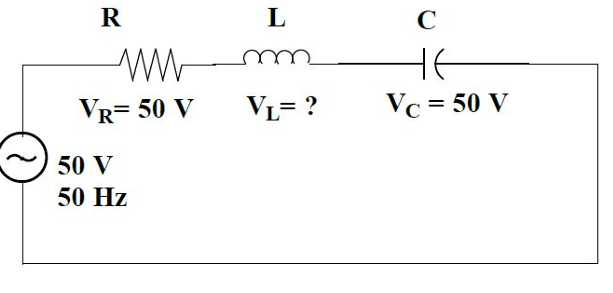
\includegraphics[width=0.5\columnwidth]{Figs/Q-6.png}
    \caption{R-L-C Circuit}
    \label{fig:placeholder_2}
\end{figure}\par \hfill\brak{\text{GATE IN 2017}}

% Q7
\item The connection of two $2$-port networks is shown in \figref{fig:placeholder_3}. The ABCD parameters of $N_1$ and $N_2$ are 
$$\myvec{A & B \\ C & D}_{N1} = \myvec{1 & 5 \\ 0 & 1}$$ and $$\myvec{A & B \\ C & D}_{N2} = \myvec{0.2 & 1 \\ 1 & 1}$$
\begin{figure}[H]
    \centering
    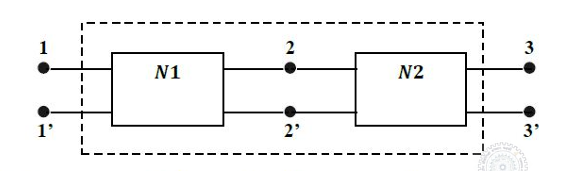
\includegraphics[width=0.5\columnwidth]{Figs/Q-7.png}
    \caption{Connection of 2-port networks}
    \label{fig:placeholder_3}
\end{figure}
The ABCD parameters of the combined 2-port network are \par \hfill\brak{\text{GATE IN 2017}}
\begin{enumerate}
\begin{multicols}{4}
    \item $\myvec{2 & 5 \\ 0.2 & 1}$
    \item $\myvec{0.5 & 1 \\ -0.5 & 1}$
    \item $\myvec{0.5 & 5 \\ 2 & 1}$
    \item $\myvec{0.5 & 5 \\ 1 & 2}$
\end{multicols}
\end{enumerate}

% Q8
\item A circuit consisting of dependent and independent sources is shown in \figref{fig:placeholder_4}. If the voltage at Node-1 is $-1$ V, then the voltage at Node-2 is \textemdash \textemdash \text{V} 
\par \hfill\brak{\text{GATE IN 2017}}
\begin{figure}[H]
    \centering
    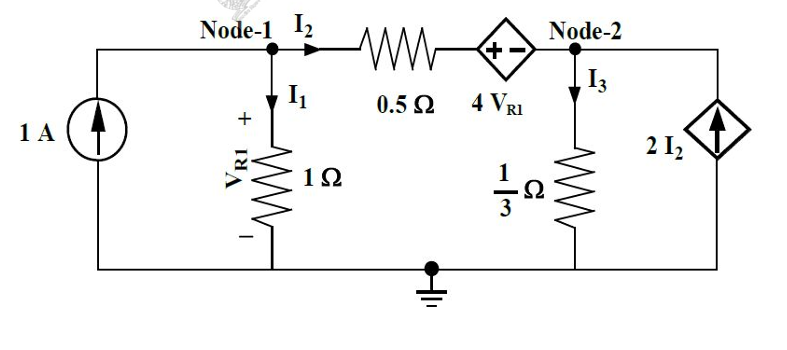
\includegraphics[width=0.6\columnwidth]{Figs/Q-8.png}
    \caption{Circuit Diagram for Question-8}
    \label{fig:placeholder_4}
\end{figure}


% Q9
\item A periodic signal $x\brak{t})$ is shown in \figref{fig:placeholder_5}. The fundamental frequency of $x\brak{t}$ in Hz is \textemdash \textemdash \par \hfill\brak{\text{GATE IN 2017}}
\begin{figure}[H]
    \centering
    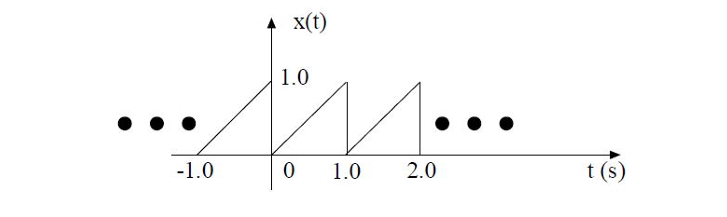
\includegraphics[width=0.7\columnwidth]{Figs/Q-9.png}
    \caption{Periodic Signal}
    \label{fig:placeholder_5}
\end{figure}

% Q10
\item A system is described by the following differential equation 
$$\frac{dy\brak{t}}{dt} + 2y\brak{t} = \frac{dx\brak{t}}{dt} + x\brak{t}, \quad x\brak{0} = y\brak{0} = 0$$
where 
$x\brak{t}$ and $y\brak{t}$ are the input and output variables respectively. The transfer function of the inverse system is \par \hfill\brak{\text{GATE IN 2017}}
\begin{enumerate}
\begin{multicols}{4}
    \item $\frac{s+1}{s-2}$
    \item $\frac{s+2}{s-1}$
    \item $\frac{s+1}{s+1}$
    \item $\frac{s+2}{s-2}$
\end{multicols}
\end{enumerate}

% Q11
\item If a continuous-time signal $x\brak{t} = \cos\brak{2\pi t}$ is sampled at $4\text{Hz}$, the value of the discrete-time sequence $x\brak{n}$ at $n=5$ is \par \hfill\brak{\text{GATE IN 2017}}
\begin{enumerate}
\begin{multicols}{4}
    \item $-0.707$
    \item $-1$
    \item $0$
    \item $1$
\end{multicols}
\end{enumerate}

% Q12
\item The Region of Convergence (ROC) of the Z-transform of a causal unit step discrete-time sequence is \par \hfill\brak{\text{GATE IN 2017}}
\begin{enumerate}
\begin{multicols}{4}
    \item $|z|<1$
    \item $|z| \leq 1$
    \item $|z| > 1$
    \item $|z| \geq 1$
\end{multicols}
\end{enumerate}

% Q13
\item The term hysteresis is associated with \par \hfill\brak{\text{GATE IN 2017}}
\begin{enumerate}
\begin{multicols}{2}
    \item ON-OFF control
    \item P-I control
    \item Feed-forward control
    \item Ratio control
\end{multicols}
\end{enumerate}

% Q14
\item The differential amplifier shown in \figref{fig:placeholder_6}, has $A_d = 100$ and common node gain of $A_c = 0.1$. If $V_1 = 5.01\text{V}$ and $V_2 = 5.00\text{V}$, then $V_o$ in volts (up to one decimal place) is \rule{1.5cm}{0.4pt} \par \hfill\brak{\text{GATE IN 2017}}
\begin{figure}[H]
    \centering
    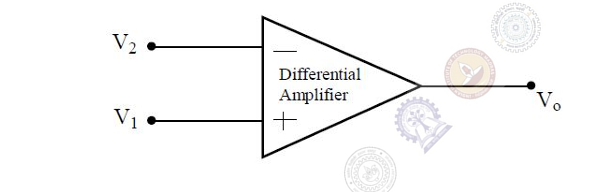
\includegraphics[width=0.7\columnwidth]{Figs/Q-14.png}
    \caption{Differential Amplifier}
    \label{fig:placeholder_6}
\end{figure}

% Q15
\item The silicon diode shown in \figref{fig:placeholder_7} has a barrier potential of $0.7\text{V}$. There will be no forward current if $V_{dc}$ in volts is greater than \par \hfill\brak{\text{GATE IN 2017}}
\begin{figure}[H]
    \centering
    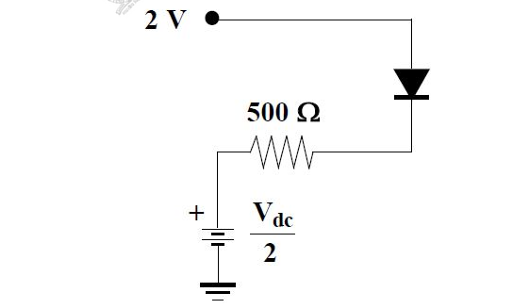
\includegraphics[width=0.5\columnwidth]{Figs/Q-15.png}
    \caption{Circuit Diagram for Question-15}
    \label{fig:placeholder_7}
\end{figure}
\begin{enumerate}
\begin{multicols}{4}
    \item $0.7$
    \item $1.3$
    \item $1.8$
    \item $2.6$
    \end{multicols}
\end{enumerate}

% Q16
\item \figref{fig:placeholder_8} shows a phase locked loop with output frequency $f_o = 5$ kHz. The value of $f_i$ in kHz is \rule{1.5cm}{0.4pt}
\par \hfill\brak{\text{GATE IN 2017}}
\begin{figure}[H] 
    \centering
    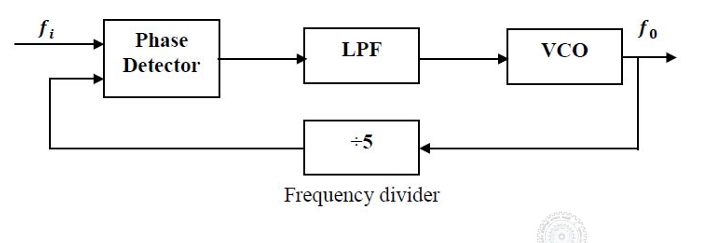
\includegraphics[width=0.7\columnwidth]{Figs/Q-16.png}
    \caption{Phase locked loop}
    \label{fig:placeholder_8}
\end{figure}

% Q17
\item The condition for oscillation in a feedback oscillator is that at the frequency pf oscillation, initially the loop gain is greater than unity while the total phase shift around the loop in degree is \par \hfill\brak{\text{GATE IN 2017}}
\begin{enumerate}
\begin{multicols}{4}
    \item $0$
    \item $90$
    \item $180$
    \item $270$
\end{multicols}
\end{enumerate}

% Q18
\item The output $V_o$ shown in \figref{fig:placeholder_9}, in volt, is closest to \par \hfill\brak{\text{GATE IN 2017}}
\begin{figure}[H]
    \centering
    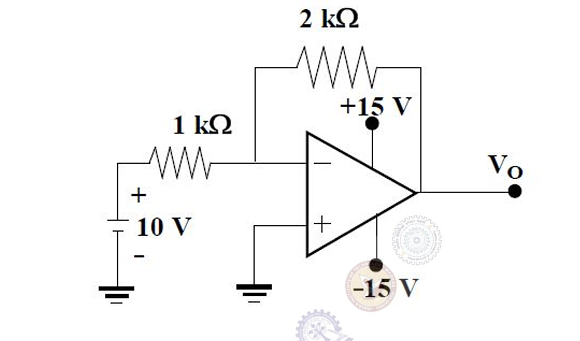
\includegraphics[width=0.5\columnwidth]{Figs/Q-18.png}
    \caption{Circuit Diagram for Question-18}
    \label{fig:placeholder_9}
\end{figure}
\begin{enumerate}
\begin{multicols}{4}
    \item $-20$
    \item $-15$
    \item $-5$
    \item $0$
\end{multicols}
\end{enumerate}

% Q19
\item An $8$-bit microcontroller with $16$ address lines has $3$ fixed interrupts i.e. Int$1$, Int$2$ and Int$3$ with corresponding interrupt vector addresses as $008$H, $0010$H and $0018$H. To execute a $32$-byte long Interrupt Service Subroutine for Int$1$ starting at the address ISS$1$, the location $0008$H onwards should ideally contain \par \hfill\brak{\text{GATE IN 2017}}
\begin{enumerate}
    \item a CALL to ISS$1$
    \item an unconditional JUMP to ISS$1$
    \item a conditional JUMP to ISS$1$
    \item only ISS$1$
\end{enumerate}

% Q20
\item A and B are the logical inputs and X is the logical output shown in \figref{fig:placeholder_10}. The output X is related to A and B by \par \hfill\brak{\text{GATE IN 2017}}
\begin{figure}[H]
    \centering
    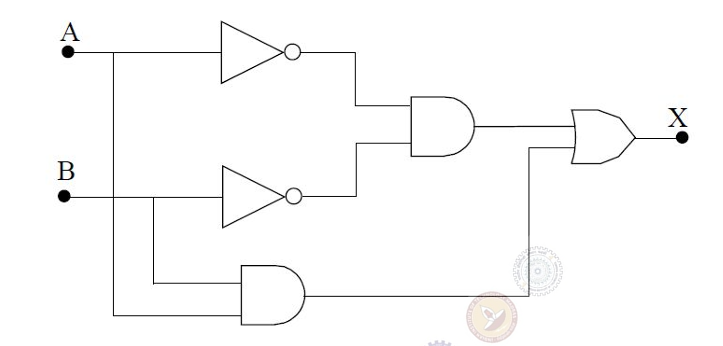
\includegraphics[width=0.6\columnwidth]{Figs/Q-20.png}
    \caption{Combination of Logic Gates}
    \label{fig:placeholder_10}
\end{figure}
\begin{enumerate}
\begin{multicols}{4}
    \item $X = \overline{A}B + B\overline{A}$
    \item $X = AB + \overline{B}A$
    \item $X = \overline{A}B + AB$
    \item $X = AB + BA$
\end{multicols}
\end{enumerate}

% Q21
\item A current waveform, $i\brak{t}$, shown in \figref{fig:placeholder_11}, is passed through a Permanent Magnet Moving Coil (PMMC) type ammeter. The reading of the ammeter up to two decimal places is \par \hfill\brak{\text{GATE IN 2017}}
\begin{figure}[H]
    \centering
    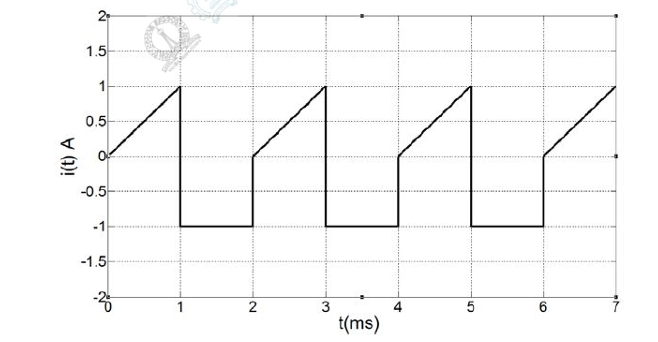
\includegraphics[width=0.5\columnwidth]{Figs/Q-21.png}
    \caption{Current Waveform}
    \label{fig:placeholder_11}
\end{figure}
\begin{enumerate}
\begin{multicols}{4}
    \item $-0.25\text{A}$
    \item $-0.12\text{A}$
    \item $0.37\text{A}$
    \item $0.50\text{A}$
\end{multicols}
\end{enumerate}

% Q22
\item Identify the instrument that does not exist \par \hfill\brak{\text{GATE IN 2017}}
\begin{enumerate}
\begin{multicols}{2}
    \item Dynamometer-type ammeter
    \item Dynamometer-type wattmeter
    \item Moving-iron voltmeter
    \item Moving-iron wattmeter
\end{multicols}
\end{enumerate}

% Q23
\item The most suitable pressure gauge to measure pressure in the range of $10^{-4}$ to $10^{-3}$ torr is  \par \hfill\brak{\text{GATE IN 2017}}
\begin{enumerate}
\begin{multicols}{4}
    \item Bellows
    \item Barometer
    \item Strain gauge
    \item Pirani gauge
\end{multicols}
\end{enumerate}

% Q24
\item The standard for long distance analog signal transmission in process control industry is \par \hfill\brak{\text{GATE IN 2017}}
\begin{enumerate}
\begin{multicols}{4}
    \item $4-20\text{mV}$
    \item $0-20\text{mA}$
    \item $4-20\text{mA}$
    \item $0-5\text{V}$
\end{multicols}
\end{enumerate}

% Q25
\item The pressure drop across an orifice plate for a particular flow rate is $5\text{kg/m}^2$. If the flow rate is doubled (withing the operating range of the orifice), the corresponding pressure drop in $\text{kg/m}^2$ is \par \hfill\brak{\text{GATE IN 2017}}
\begin{enumerate}
\begin{multicols}{4}
    \item $2.5$
    \item $5.0$
    \item $20.0$
    \item $25.0$
\end{multicols}
\end{enumerate}

% Q26
\item The probability that a communication system will have high fidelity is $0.81$. The probability that the system will have both high fidelity and high selectivity is $0.18$. The probability that a given system with high fidelity will have high selectivity is \par \hfill\brak{\text{GATE IN 2017}}
\begin{enumerate}
\begin{multicols}{4}
    \item $0.181$
    \item $0.191$
    \item $0.222$
    \item $0.826$
\end{multicols}
\end{enumerate}

% Q27
\item The angle between two vectors $\textbf{x}_1 = [2\quad 6\quad 14]^T$ and $x_2 = [-12\quad 8\quad 16]^T$ in radian is \rule{1.5cm}{0.4pt} 
\par \hfill\brak{\text{GATE IN 2017}}

% Q28
\item The following table lists an $n^\text{th}$ order polynomial $f(x) = a_n x^n + a_{n-1} x^{n-1} + \dots + a_1 x + a_0$ and the forward differences evaluated at equally spaced values of $x$. The order of the polynomial is \par \hfill\brak{\text{GATE IN 2017}}

\begin{table}[H]
    \centering
    \begin{center}
\begin{tabular}{|c|c|c|}
\hline
\textbf{Mineral} & \textbf{Entropy $S^{1,823}$ (kJ K$^{-1}$)} & \textbf{Volume $V^{1,823}$ (J bar$^{-1}$)} \\
\hline
Grossular   & 0.255 & 12.535 \\
\hline
Quartz      & 0.042 & 2.269 \\
\hline
Anorthite   & 0.200 & 10.079 \\
\hline
Wollastonite & 0.082 & 3.993 \\
\hline
\end{tabular}    
\end{center}



\end{table}

\begin{enumerate}
\begin{multicols}{4}
    \item $1$
    \item $2$
    \item $3$
    \item $4$
\end{multicols}
\end{enumerate}

% Q29
\item The current response of a series R-L circuit to a unit step voltage is given in the table. The value of $\text{L}$ is \rule{1.5cm}{0.4pt} \textbf{H}. \par \hfill\brak{\text{GATE IN 2017}}
\begin{table}[H]
    \centering
    \setlength{\fboxsep}{6pt} % padding inside the box

\begin{center}
\fbox{%
  \begin{minipage}{0.96\textwidth}
    \underline{\textbf{Useful data}}\\[6pt]

    \begin{tabular}{l l}
      Avogadro's Number & : $6.023\times10^{23}\ \mathrm{mol^{-1}}$\\[4pt]
      Boltzmann's constant & : $1.38\times10^{-23}\ \mathrm{J\ K^{-1}}$\\[4pt]
      Electron Charge & : $1.6\times10^{-19}\ \mathrm{C}$\\[4pt]
      Gas Constant & : $8.314\ \mathrm{J\ mol^{-1}\ K^{-1}}$\\[4pt]
      Electron rest mass & : $9.1\times10^{-31}\ \mathrm{kg}$\\[4pt]
      Permittivity of vacuum ($\varepsilon_0$) & : $8.854\times10^{-12}\ \mathrm{F\ m^{-1}}$\\[4pt]
      Planck's constant ($h$) & : $6.62\times10^{-34}\ \mathrm{J\ s^{-1}}$\\[4pt]
      Bohr Magneton ($\mu_B$) & : $9.27\times10^{-24}\ \mathrm{A\ m^{2}}$\\
    \end{tabular}

    \vspace{8pt}

    $1\ \mathrm{eV} = 1.6\times10^{-19}\ \mathrm{J}$\\[2pt]
    $1\ \mathrm{cal} = 4.2\ \mathrm{J}$

    \vspace{10pt}

    \textbf{Atomic weight (in kg mol$^{-1}$) of:}\\[6pt]
    \begin{tabular}{l l}
      Hydrogen & 0.001\\
      Carbon   & 0.012\\
      Nitrogen & 0.014
    \end{tabular}

  \end{minipage}%
}%
\end{center}

\end{table}

% Q30
\item For the circuit shown in \figref{fig:placeholder_12}, the total real power delivered by the source to the loads is \rule{1.5cm}{0.4pt} $\textbf{kW}$. \par \hfill\brak{\text{GATE IN 2017}}
\begin{figure}[H]
    \centering
    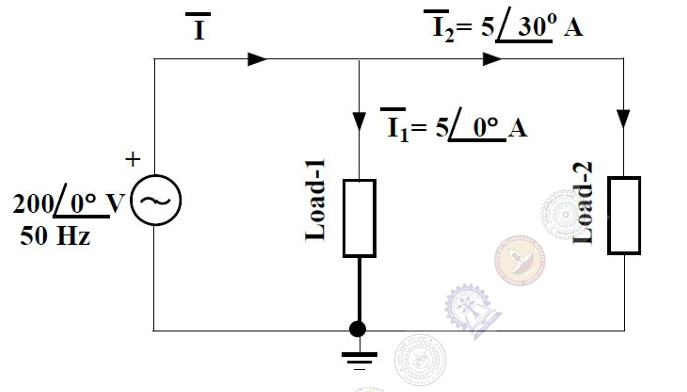
\includegraphics[width=0.5\columnwidth]{Figs/Q-30.png}
    \caption{Circuit Diagram for Question-30}
    \label{fig:placeholder_12}
\end{figure}


% Q31
\item A series R-L-C circuit is excited with an a.c. voltage source. The quality factor $\brak{\text{Q}}$ is $\text{Q} = 30$. The amplitude of current in amperes at the upper half-power frequency will be \rule{1.5cm}{0.4pt}. \par \hfill\brak{\text{GATE IN 2017}}
\begin{figure}[H]
    \centering
    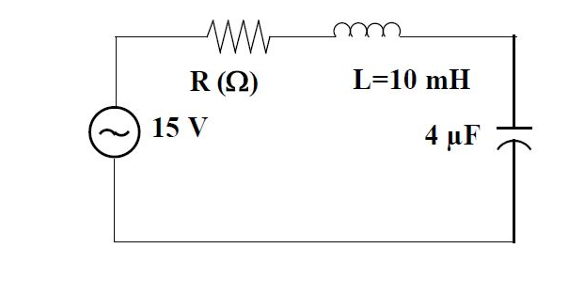
\includegraphics[width=0.5\columnwidth]{Figs/Q-31.png}
    \caption{R-L-C Circuit}
    \label{fig:placeholder_13}
\end{figure}

% Q32
\item In the circuit (\figref{fig:placeholder_14} shown, $S_1$ was closed and $S_2$ was open for a very long time. At $t=0$, $S_1$ is opened and $S_2$ is closed. The voltage across the capacitor at $t = 5 \ \mu\text{s}$ is \rule{1.5cm}{0.4pt} $\text{V}$. \par \hfill\brak{\text{GATE IN 2017}}
\begin{figure}[H]
    \centering
    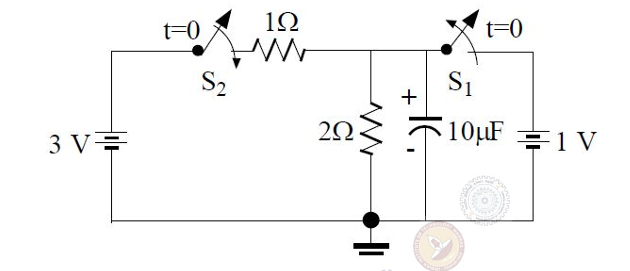
\includegraphics[width=0.6\columnwidth]{Figs/Q-32.png}
    \caption{Circuit Diagram for Question-32}
    \label{fig:placeholder_14}
\end{figure}

% Q33
\item Consider two discrete-time signals   
$x_1\brak{n} = \cbrak{1, 1}$ and $x_2 \brak{n} = \{1, 2\}$ for $n = 0, 1$.\\ 
The Z-transform of $x \brak{n} = x_1 \brak{n} * x_2 \brak{n}$ is \par \hfill\brak{\text{GATE IN 2017}}
\begin{enumerate}
\begin{multicols}{4}
    \item $1 + 2z^{-1} + 3z^{-2}$
    \item $z^2 + 3z + 2$
    \item $1 + 3z^{-1} + 2z^{-2}$
    \item $z^{-2} + 3z^{-3} + 2z^{-4}$
\end{multicols}
\end{enumerate}

% Q34
\item Three DFT coefficients, out of five DFT coefficients of a five-point real sequence are given as $X \brak{0} = 4$, $X \brak{1} = 1 - j1$, $X \brak{3} = 2 + j2$.  
The zero-th value of the sequence $x\brak{n}$, $x \brak{0}$, is \par \hfill\brak{\text{GATE IN 2017}}
\begin{enumerate}
\begin{multicols}{4}
    \item 1
    \item 2
    \item 3
    \item 4
\end{multicols}
\end{enumerate}

% Q35
\item The Laplace transform of a causal signal $y\brak{t}$ is $Y \brak{s} = \frac{s+2}{s+6}.$  
The value of $y\brak{t}$ at $t = 0.1$ s is \rule{1.5cm}{0.4pt}. \par \hfill\brak{\text{GATE IN 2017}}

% Q36
\item The block diagram of a closed-loop control system is shown in \figref{fig:placeholder_15}. The values of $k$ and $k_p$ are such that the system has a damping ratio of $0.8$ and an undamped frequency $\omega_n$ of $4\text{rad/s}$ respectively. The value of $k_p$ will be \rule{1.5cm}{0.4pt}. \par \hfill\brak{\text{GATE IN 2017}}
\begin{figure}[H]
    \centering
    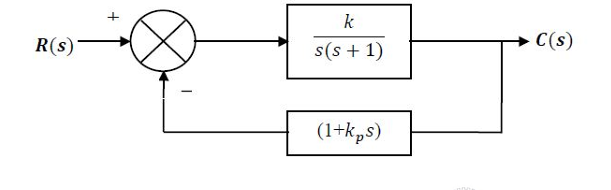
\includegraphics[width=0.6\columnwidth]{Figs/Q-36.png}
    \caption{Block diagram of a closed loop control system}
    \label{fig:placeholder_15}
\end{figure}


% Q37
\item The loop transfer function of a closed-loop system is given by $G \brak{s}H \brak{s} = \frac{K(s+6)}{s(s+2)}.$ 
The breakaway point of the root-loci will be \rule{1.5cm}{0.4pt}. \par \hfill\brak{\text{GATE IN 2017}}

% Q38
\item The closed-loop system shown in \figref{fig:placeholder_16}. The system parameter $\alpha$ is not known. They condition for asymptotic stability of the closed loop system is \par \hfill\brak{\text{GATE IN 2017}}
\begin{figure}[H]
    \centering
    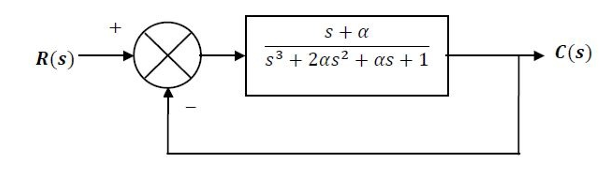
\includegraphics[width=0.6\columnwidth]{Figs/Q-38.png}
    \caption{Closed loop system}
    \label{fig:placeholder_16}
\end{figure}
\begin{enumerate}
\begin{multicols}{4}
    \item $\alpha < -0.5$
    \item $-0.5 < \alpha < 0.5$
    \item $0 < \alpha < 0.5$
    \item $\alpha > 0.5$
\end{multicols}
\end{enumerate}

% Q39 
\item The overall closed-loop transfer function $\frac{C(s)}{R(s)}$, represented in \figref{fig:placeholder_17}, will be \par \hfill\brak{\text{GATE IN 2017}}
\begin{figure}[H]
    \centering
    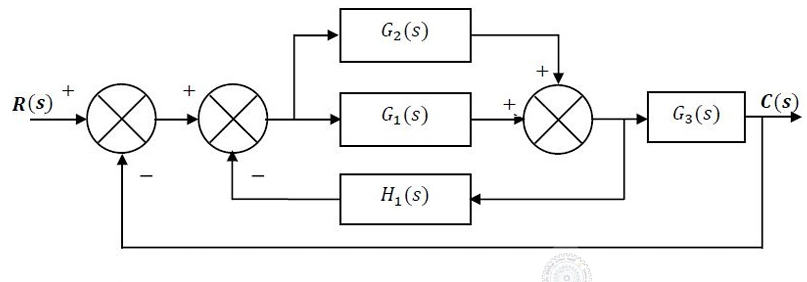
\includegraphics[width=0.7\columnwidth]{Figs/Q-39.png}
    \caption{Closed loop system}
    \label{fig:placeholder_17}
\end{figure}
\begin{enumerate}
\begin{multicols}{2}
    \item $\frac{\brak{G_1\brak{s}+G_2\brak{s}}G_3\brak{s}}{1+\brak{G_1\brak{s}+G_2\brak{s}}\brak{H_1\brak{s}+G_3\brak{s}}}$
    \item $\frac{\brak{G_1\brak{s}+G_3\brak{s}}}{1+G_1\brak{s}H_1+\brak{s}+G_2\brak{s}G_3\brak{s}}$
    \item $\frac{\brak{G_1\brak{s}-G_2\brak{s}}H_1\brak{s}}{1+\brak{G_1\brak{s}+G_3\brak{s}}\brak{H_1\brak{s}+G_1\brak{s}}}$
    \item $\frac{G_1\brak{s}G_2\brak{s}H_1\brak{s}}{1+G_1\brak{s}H_1+\brak{s}+G_1\brak{s}G_3\brak{s}}$
\end{multicols}
\end{enumerate}

% Q40
\item Assuming the op-amp shown in \figref{fig:placeholder_18} to be ideal, the frequency at which $|V_0|$ will be $95\%$ of $V_{\text{in}}$ is \rule{1.5cm}{0.4pt} $\text{kHz}$. \par \hfill\brak{\text{GATE IN 2017}}
\begin{figure}[H]
    \centering
    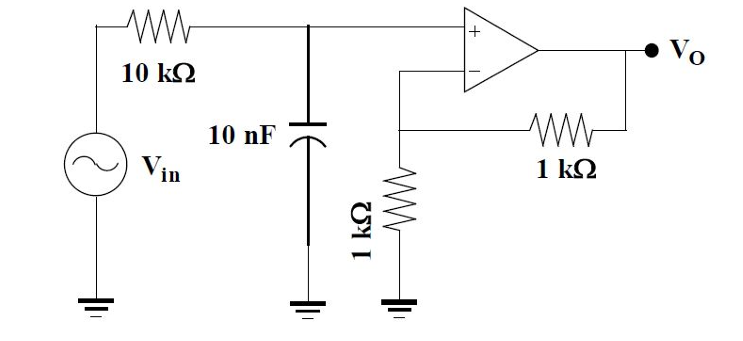
\includegraphics[width=0.6\columnwidth]{Figs/Q-40.png}
    \caption{Circuit Diagram for Question-40}
    \label{fig:placeholder_18}
\end{figure}

% Q41
\item In the circuit, shown in \figref{fig:placeholder_19}, The MOSFET operates in the saturation zone. The characteristics of the MOSFET is given by $I_D = \frac{1}{2}(V_{GS} - 1)^2\text{mA}$. For $V_S = +5\text{V}$, $R_S$ in $\text{k}\ohm$ is \rule{1.5cm}{0.4pt}. \par \hfill\brak{\text{GATE IN 2017}}
\begin{figure}[H]
    \centering
    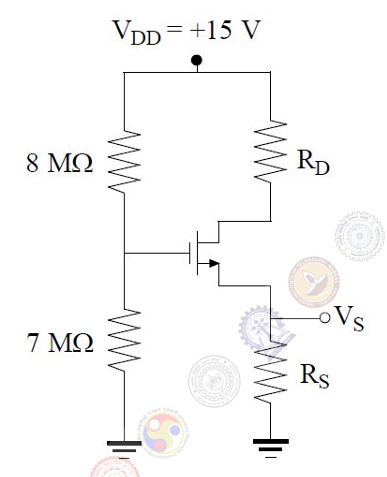
\includegraphics[width=0.4\columnwidth]{Figs/Q-41.png}
    \caption{Circuit Diagram for Question-41}
    \label{fig:placeholder_19}
\end{figure}

% Q42
\item The two-input voltage multiplier, shown in \figref{fig:placeholder_20}, has a scaling factor of $1$ and produces voltage output. If $V_1 = +15\text{V}$ and $V_2 = +3\text{V}$, the value of $V_o$ in \textbf{volt} is \rule{1.5cm}{0.4pt}. \par \hfill\brak{\text{GATE IN 2017}}
\begin{figure}[H]
    \centering
    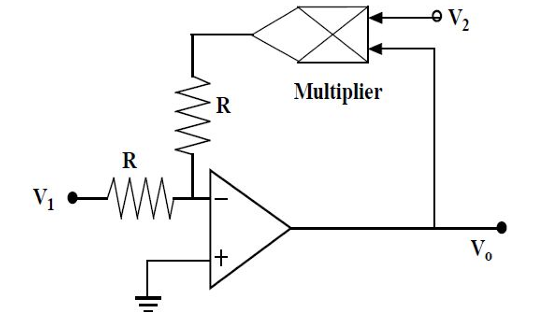
\includegraphics[width=0.5\columnwidth]{Figs/Q-42.png}
    \caption{Circuit Diagram for Question-42}
    \label{fig:placeholder_20}
\end{figure}


% Q43
\item The two inputs A and B are connected to an R-S latch via two AND gates as shown in \figref{fig:placeholder_21}. If $\text{A}=1$ and $\text{B}=0$, the output $Q\overline{Q}$ is \par \hfill\brak{\text{GATE IN 2017}}
\begin{figure}[H]
    \centering
    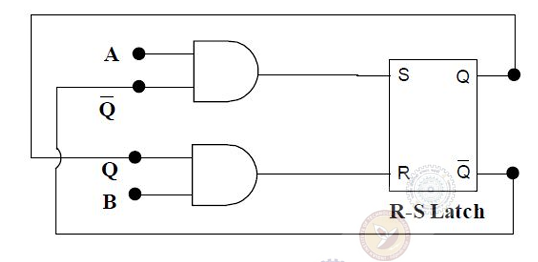
\includegraphics[width=0.5\columnwidth]{Figs/Q-43.png}
    \caption{Combination of AND Gates}
    \label{fig:placeholder_21}
\end{figure}
\begin{enumerate}
\begin{multicols}{4}
    \item 00
    \item 10
    \item 01
    \item 11  
\end{multicols}
\end{enumerate}

% Q44
\item The circuit of a Schmitt trigger is shown in \figref{f-21}. The zener-diode combination maintains the output between $\pm 7\text{V}$. The width of the hysteresis bandis \rule{1.5cm}{0.4pt} $\text{V}$. \par \hfill\brak{\text{GATE IN 2017}}
\begin{figure}[H]
    \centering
    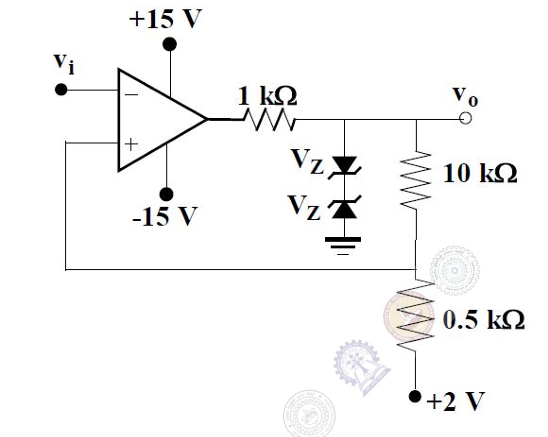
\includegraphics[width=0.5\columnwidth]{Figs/Q-44.png}
    \caption{Closed loop system}
    \label{f-21}
\end{figure}

% Q45
\item When the voltage across a battery is measured using a d.c. potentiometer, the reading
shows $1.08 \text{V}$. But when the same voltage is measured using a Permanent Magnet Moving
Coil (PMMC) voltmeter, the voltmeter reading shows $0.99 \text{V}$. If the resistance of the
voltmeter is $1100 \ohm$, the internal resistance of the battery, in $\ohm$, is \rule{1.5cm}{0.4pt}. \par \hfill\brak{\text{GATE IN 2017}}

% Q46
\item The power delivered to a single phase inductive load is measured with a dynamometer type wattmeter using a potential transformer (PT) of turns ratio 200:1 and the current
transformer (CT) of turns ratio $1$:$5$. Assume both the transformers to be ideal. The power
factor of the load is $0.8$. If the wattmeter reading is $200 \text{W}$, then the apparent power of the load in $\textbf{kVA}$ is \rule{1.5cm}{0.4pt}. \par \hfill\brak{\text{GATE IN 2017}}

%47
\item The unbalanced voltage of the Wheatstone bridge, shown in \figref{f-22}, is measured using a digital voltmeter having infinite input impedance and a resolution of $0.1 \textbf{mV}$. If $R=10000\ohm$, the minimum value of $\Delta R$ in $\ohm$ to create a detectable unbalanced voltage is \rule{1.5cm}{0.4pt}. \par \hfill\brak{\text{GATE IN 2017}}
\begin{figure}[H]
    \centering
    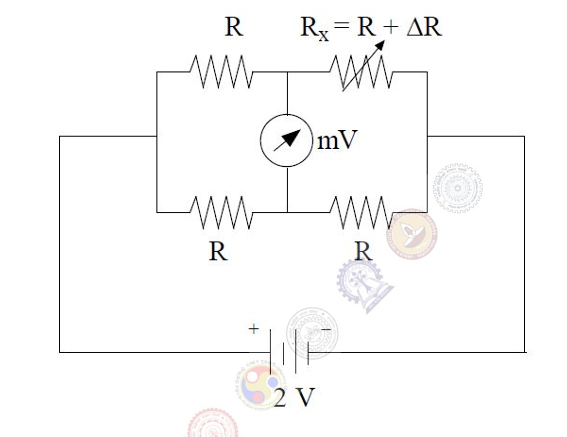
\includegraphics[width=0.5\columnwidth]{Figs/Q-47.png}
    \caption{Wheatstone Bridge}
    \label{f-22}
\end{figure}

%48
\item In the a.c. bridge, shown in \figref{f-23}, $R = 10^{3}\ \ohm$ and $C = 10^{-7}\text{F}$. If the bridge is balanced at a frequency $\omega_0$, the value of $\omega_0$ in $\text{rad/s}$ is \rule{1.5cm}{0.4pt}. \par \hfill\brak{\text{GATE IN 2017}}
\begin{figure}[H]
    \centering
    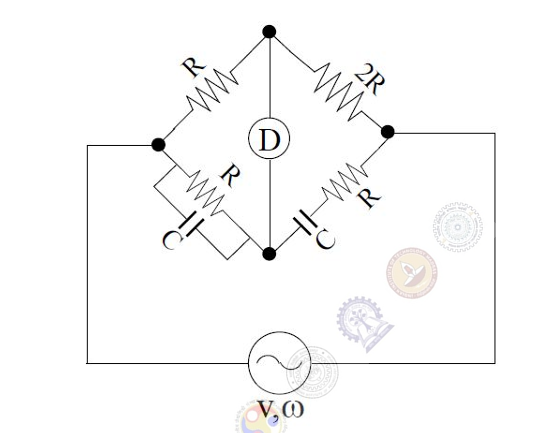
\includegraphics[width=0.6\columnwidth]{Figs/Q-48.png}
    \caption{AC Bridge}
    \label{f-23}
\end{figure}

%49
\item The hot junction of a bare thermocouple, initially at room temperature $\brak{30\degree\text{C}}$, is suddenly
dipped in molten metal at $t = 0s$. The cold junction is kept at room temperature. The
thermocouple can be modeled as a first-order instrument with a time constant of $1.0 s$ and a
static sensitivity of $10{\mu}\text{V}/{\degree}\text{C}$. If the voltage measured across the thermocouple indicates
$10.0 mV$ at $t = 1.0s$ , then the temperature of the molten metal in ${\degree}\text{C}$ is \rule{1.5cm}{0.4pt} \par \hfill\brak{\text{GATE IN 2017}}

% Q50
\item A resistance temperature detector (RTD) is connected to a circuit, as shown in \figref{f-24}.
Assume the opamp to be ideal. If $V = +2.0\text{V}$, then the value of $x$ is \rule{1.5cm}{0.4pt}. \par \hfill\brak{\text{GATE IN 2017}}
\begin{figure}[H]
    \centering
    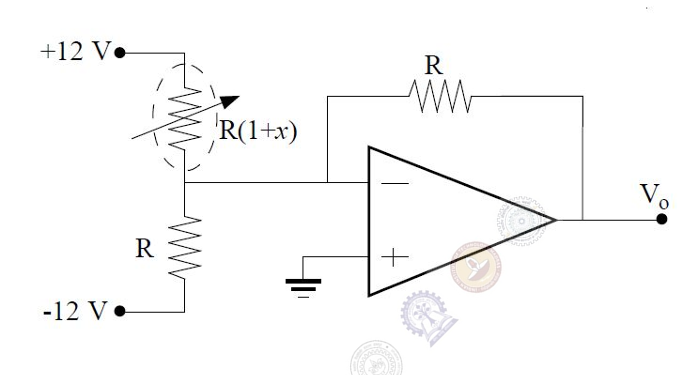
\includegraphics[width=0.6\columnwidth]{Figs/Q-50.png}
    \caption{Circuit Diagram for Question-50}
    \label{f-24}
\end{figure}


% Q51
\item The magnetic flux density of an electromagnetic flowmeter is $100 \text{mWb}/{m}^2$. The electrodes are wall-mounted inside the pipe having a diameter of $0.25\text{m}$. A voltage of $1 \text{V}$ is generated when a conducting fluid is passed through the flowmeter. The volumetric flowrate of the fluid in $m^3/s$ is \rule{1.5cm}{0.4pt}. \par \hfill\brak{\text{GATE IN 2017}}

% Q52
\item The junction semiconductor temperature sensor shown in \figref{f-25} is used to measure the temperature of hot air. The output voltage $V_o$ is $2.1 \text{V}$. The current output of the sensor is given by $I = T \mu\text{A}$ where $T$ is the temperature in $\text{K}$. Assuming the opamp to be ideal, the temperature of the hot air in $\degree\text{C}$ is approximately \rule{1.5cm}{0.4pt}. \par \hfill\brak{\text{GATE IN 2017}}
\begin{figure}[H]
    \centering
    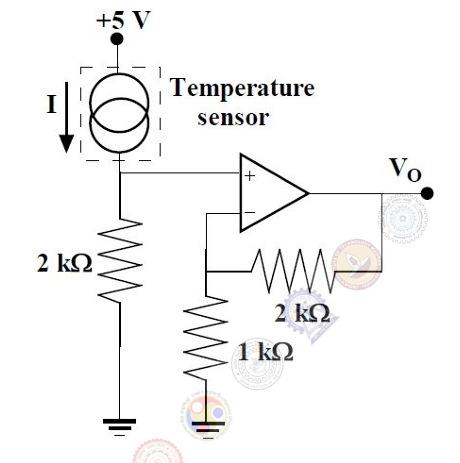
\includegraphics[width=0.6\columnwidth]{Figs/Q-52.png}
    \caption{Circuit Diagram for Question-52}
    \label{f-25}
\end{figure}

% Q53
\item Quantum efficiency of a photodiode (ratio between the number of liberated electrons and
the number of incident photons) is $0.75$ at $830 \text{nm}$. Given Planck's constant
$h = 6.624 \times 10^{-34}\text{J}$, the charge of an electron $e = 1.6 \times 10^{-19}\text{C}$ and the velocity of
light in the photodiode $C_m = 2 \times 10^{8}\text{m/s}$. For an incident optical power of $100$ $\mu\text{W}$ at
$830 \text{nm}$, the photocurrent in $\mu\text{A}$ is \rule{1.5cm}{0.4pt}. \par \hfill\brak{\text{GATE IN 2017}}

% Q54
\item In a sinusoidal amplitude modulation scheme (with carrier) the modulated signal is given
by $A_m\brak{t} = 100 \cos\brak{\omega_c t} + 50 \cos\brak{\omega_m t} \cos\brak{\omega_c t}$,
where $\omega_c$ is the carrier frequency and
$\omega_m$ is the modulation frequency. The power carried by the sidebands in \% of total power is \rule{1.5cm}{0.4pt} \% \par \hfill\brak{\text{GATE IN 2017}}

% Q55
\item An angle modulated signal with carrier frequency $\omega_c = 2\pi \times10^6\text{rad/s}$ is given by  
$4m(t) = \cos\brak{\omega_c t + 5 \sin\brak{1000\pi t} + 10 \sin\brak{2000 \pi t}}$.  
The maximum deviation of the frequency in the angle modulated signal from that of the carrier is \rule{1.5cm}{0.4pt} $\text{kHz}$. \par \hfill\brak{\text{GATE IN 2017}}

% Q56
\item The event would have been successful if you \rule{1.5cm}{0.4pt} able to come. \par \hfill\brak{\text{GATE IN 2017}}
\begin{enumerate}
\begin{multicols}{4}
    \item are
    \item had been
    \item have been
    \item would have been
\end{multicols}
\end{enumerate}

% Q57
\item There was no doubt that their work was \underline{thorough}.  
Which of the words below is closest in meaning to the underlined word above? \par \hfill\brak{\text{GATE IN 2017}}
\begin{enumerate}
\begin{multicols}{4}
    \item pretty
    \item complete
    \item sloppy
    \item haphazard
\end{multicols}
\end{enumerate}

% Q58
\item Four cards lie on a table. Each card has a number printed on one side and a colour on the other. The faces visible on the cards are $2$, $3$, red, and blue. 
Proposition: If a card has an even value on one side, then its opposite face is red.  
The cards which MUST be turned over to verify the above proposition are \par \hfill\brak{\text{GATE IN 2017}}
\begin{enumerate}
\begin{multicols}{4}
    \item $2$, red
    \item $2$, $3$, red
    \item $2$, blue
    \item $2$, red, blue
\end{multicols}
\end{enumerate}

% Q59
\item What is the value of $x$ when  
$$81 \times \frac{x+2}{16} \div \frac{2x+4}{25} = 144\ ?$$ \par \hfill\brak{\text{GATE IN 2017}}
\begin{enumerate}
\begin{multicols}{4}
    \item 1
    \item -1
    \item -2
    \item Cannot be determined
\end{multicols}
\end{enumerate}

% Q60
\item Two dice are thrown simultaneously. The probability that the product of the numbers appearing on
the top faces of the dice is a perfect square is \par \hfill\brak{\text{GATE IN 2017}}
\begin{enumerate}
\begin{multicols}{4}
    \item $\frac{1}{9}$
    \item $\frac{2}{9}$
    \item $\frac{1}{3}$
    \item $\frac{4}{9}$
\end{multicols}
\end{enumerate}

% Q61
\item Bhaichung was observing the pattern of people entering and leaving a car service centre. There was a single window where customers were being served. He saw that people inevitably came out of the centre in the order that they went in. However, the time they spent inside seemed to vary a lot: some people came out in a matter of minutes while for others it took much longer.

From this, what can one conclude? \par \hfill\brak{\text{GATE IN 2017}}
\begin{enumerate}
    \item The centre operates on a first-come-first-served basis, but with variable service times, depending on specific customer needs.
    \item Customers were served in an arbitrary order, since they took varying amounts of time for service completion in the centre.
    \item Since some people came out within a few minutes of entering the centre, the system is likely to operate on a last-come-first-served basis.
    \item Entering the centre early ensured that one would have shorter service times and most people attempted to do this.
\end{enumerate}

% Q62
\item A map shows the elevations of Darjeeling, Gangtok, Kalimpong, Pelling, and Siliguri.
Kalimpong is at a lower elevation than Gangtok. Pelling is at a lower elevation than Gangtok.
Pelling is at a higher elevation than Siliguri. Darjeeling is at a higher elevation than Gangtok.

Which of the following statements can be inferred from the paragraph above?

i. Pelling is at a higher elevation than Kalimpong \\
ii. Kalimpong is at a lower elevation than Darjeeling \\
iii. Kalimpong is at a higher elevation than Siliguri \\
iv. Siliguri is at a lower elevation than Gangtok
\par \hfill\brak{\text{GATE IN 2017}}

\begin{enumerate}
\begin{multicols}{4}
    \item Only ii
    \item Only ii and iii
    \item Only ii and iv
    \item Only iii and iv
\end{multicols}
\end{enumerate}

% Q63
\item P, Q, R, S, T and U are seated around a circular table. R is seated two places to the right of Q. P is
seated three places to the left of R. S is seated opposite U. If P and U now switch seats, which of
the following must necessarily be true?
\par \hfill\brak{\text{GATE IN 2017}}
\begin{enumerate}
    \item P is immediately to the right of R
    \item T is immediately to the left of P
    \item T is immediately to the left of P or P is immediately to the right of Q
    \item U is immediately to the right of R or P is immediately to the left of T
\end{enumerate}

% Q64
\item Budhan covers a distance of $19 \brak{km}$ in $2$ hours by cycling one fourth of the time and walking the rest. The next day he cycles (at the same speed as before) for half the time and walks the rest (at the same speed as before) and covers $26 \brak{km}$ in 2 hours. The speed in km/h at which Budhan walks is \par \hfill\brak{\text{GATE IN 2017}}
\begin{enumerate}
\begin{multicols}{4}
    \item 1
    \item 4
    \item 5
    \item 6
\end{multicols}
\end{enumerate}

% Q65
\item The points in the graph below (\figref{f-26}) represent the halts of a lift for durations of $1$ minute, over a period of
$1$ hour. \par \hfill\brak{\text{GATE IN 2017}}
\begin{figure}[H]
    \centering
    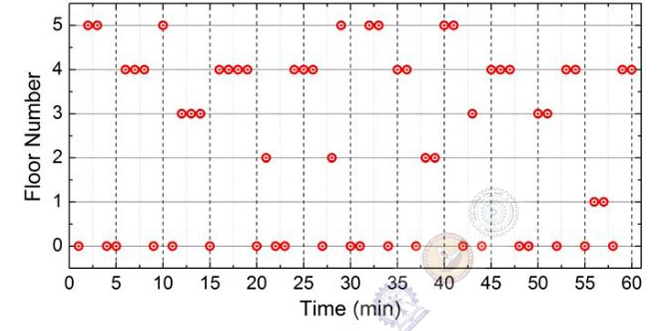
\includegraphics[width=0.7\columnwidth]{Figs/Q-65.png}
    \caption{Halts of a lift}
    \label{f-26}
\end{figure}

Which of the following statements are correct? \\
i. The elevator never moves directly from any non-ground floor to another non-ground floor over the one hour period\\
ii. The elevator stays on the fourth floor for the longest duration over the one hour period

\begin{enumerate}
\begin{multicols}{4}
    \item Only i
    \item Only ii
    \item Both i and ii
    \item Neither i nor ii
\end{multicols}
\end{enumerate}


\end{enumerate}

\end{document}
